\documentclass[twoside]{book}

% Packages required by doxygen
\usepackage{fixltx2e}
\usepackage{calc}
\usepackage{doxygen}
\usepackage[export]{adjustbox} % also loads graphicx
\usepackage{graphicx}
\usepackage[utf8]{inputenc}
\usepackage{makeidx}
\usepackage{multicol}
\usepackage{multirow}
\PassOptionsToPackage{warn}{textcomp}
\usepackage{textcomp}
\usepackage[nointegrals]{wasysym}
\usepackage[table]{xcolor}

% Font selection
\usepackage[T1]{fontenc}
\usepackage[scaled=.90]{helvet}
\usepackage{courier}
\usepackage{amssymb}
\usepackage{sectsty}
\renewcommand{\familydefault}{\sfdefault}
\allsectionsfont{%
  \fontseries{bc}\selectfont%
  \color{darkgray}%
}
\renewcommand{\DoxyLabelFont}{%
  \fontseries{bc}\selectfont%
  \color{darkgray}%
}
\newcommand{\+}{\discretionary{\mbox{\scriptsize$\hookleftarrow$}}{}{}}

% Page & text layout
\usepackage{geometry}
\geometry{%
  a4paper,%
  top=2.5cm,%
  bottom=2.5cm,%
  left=2.5cm,%
  right=2.5cm%
}
\tolerance=750
\hfuzz=15pt
\hbadness=750
\setlength{\emergencystretch}{15pt}
\setlength{\parindent}{0cm}
\setlength{\parskip}{3ex plus 2ex minus 2ex}
\makeatletter
\renewcommand{\paragraph}{%
  \@startsection{paragraph}{4}{0ex}{-1.0ex}{1.0ex}{%
    \normalfont\normalsize\bfseries\SS@parafont%
  }%
}
\renewcommand{\subparagraph}{%
  \@startsection{subparagraph}{5}{0ex}{-1.0ex}{1.0ex}{%
    \normalfont\normalsize\bfseries\SS@subparafont%
  }%
}
\makeatother

% Headers & footers
\usepackage{fancyhdr}
\pagestyle{fancyplain}
\fancyhead[LE]{\fancyplain{}{\bfseries\thepage}}
\fancyhead[CE]{\fancyplain{}{}}
\fancyhead[RE]{\fancyplain{}{\bfseries\leftmark}}
\fancyhead[LO]{\fancyplain{}{\bfseries\rightmark}}
\fancyhead[CO]{\fancyplain{}{}}
\fancyhead[RO]{\fancyplain{}{\bfseries\thepage}}
\fancyfoot[LE]{\fancyplain{}{}}
\fancyfoot[CE]{\fancyplain{}{}}
\fancyfoot[RE]{\fancyplain{}{\bfseries\scriptsize Generated by Doxygen }}
\fancyfoot[LO]{\fancyplain{}{\bfseries\scriptsize Generated by Doxygen }}
\fancyfoot[CO]{\fancyplain{}{}}
\fancyfoot[RO]{\fancyplain{}{}}
\renewcommand{\footrulewidth}{0.4pt}
\renewcommand{\chaptermark}[1]{%
  \markboth{#1}{}%
}
\renewcommand{\sectionmark}[1]{%
  \markright{\thesection\ #1}%
}

% Indices & bibliography
\usepackage{natbib}
\usepackage[titles]{tocloft}
\setcounter{tocdepth}{3}
\setcounter{secnumdepth}{5}
\makeindex

% Hyperlinks (required, but should be loaded last)
\usepackage{ifpdf}
\ifpdf
  \usepackage[pdftex,pagebackref=true]{hyperref}
\else
  \usepackage[ps2pdf,pagebackref=true]{hyperref}
\fi
\hypersetup{%
  colorlinks=true,%
  linkcolor=blue,%
  citecolor=blue,%
  unicode%
}

% Custom commands
\newcommand{\clearemptydoublepage}{%
  \newpage{\pagestyle{empty}\cleardoublepage}%
}

\usepackage{caption}
\captionsetup{labelsep=space,justification=centering,font={bf},singlelinecheck=off,skip=4pt,position=top}

%===== C O N T E N T S =====

\begin{document}

% Titlepage & ToC
\hypersetup{pageanchor=false,
             bookmarksnumbered=true,
             pdfencoding=unicode
            }
\pagenumbering{alph}
\begin{titlepage}
\vspace*{7cm}
\begin{center}%
{\Large C\+S1\+Cofficial \\[1ex]\large 0.\+5 }\\
\vspace*{1cm}
{\large Generated by Doxygen 1.8.14}\\
\end{center}
\end{titlepage}
\clearemptydoublepage
\pagenumbering{roman}
\tableofcontents
\clearemptydoublepage
\pagenumbering{arabic}
\hypersetup{pageanchor=true}

%--- Begin generated contents ---
\chapter{C\+S1\+Cproject}
\label{md__r_e_a_d_m_e}
\Hypertarget{md__r_e_a_d_m_e}
2D Render Application

Goals\+: 1) Provide “contact us” method with team name and logo

2) Display all graphic objects (i.\+e. shapes including text) in rendering window. The shape id will be displayed above each shape identifying it. The rendering area to display shapes must have minimum dimensions of 1000 pixels (horizontal) by 500 pixels (vertical). The coordinate system is defined such that the top left corner of the rendering area is located at point (0,0), the bottom right corner at point (1000,500).

3) Your program should read from a shape file that keeps track of all shapes currently being rendered by the 2D modeler. Shapes are identified by their type\+: line, polyline, polygon, rectangle, ellipse, text. Shapes have properties\+: shape dimensions, pen color, pen width, pen style, pen cap style, pen join style, brush color, brush shape. \mbox{\hyperlink{class_text}{Text}} has properties\+: shape dimensions, text string, text color, text alignment, text point size, text font family, text font style, text font weight. All shapes must also have a unique ID.

4) Your program should be able to move shapes, including text, being rendered. This is accomplished via a move shape form. All changes are visible in the rendering area. –administrator only

5) Your program should be able to add and removeshapes, including text, being rendered.\+This is accomplished via an add/remove shape form. All changes are visible in the rendering area. –administrator only

6) Produce a shape listing report sorted by shape id (at any time). All shape properties should be included in the report.

7) Produce a shape listing report of O\+N\+LY shapes with an area sorted by area (at any time). The shape type, id and area should be included in the report.

8) Produce a shape listing report of O\+N\+LY shapes with a perimeter sorted by perimeter (at any time). The shape type, id and perimeter should be included in the report.

9) Save all changes between executions 
\chapter{Hierarchical Index}
\section{Class Hierarchy}
This inheritance list is sorted roughly, but not completely, alphabetically\+:\begin{DoxyCompactList}
\item Q\+Dialog\begin{DoxyCompactList}
\item \contentsline{section}{contact}{\pageref{classcontact}}{}
\item \contentsline{section}{log\+In}{\pageref{classlog_in}}{}
\end{DoxyCompactList}
\item Q\+Main\+Window\begin{DoxyCompactList}
\item \contentsline{section}{Main\+Window}{\pageref{class_main_window}}{}
\end{DoxyCompactList}
\item Q\+Widget\begin{DoxyCompactList}
\item \contentsline{section}{Render\+Area}{\pageref{class_render_area}}{}
\item \contentsline{section}{Window}{\pageref{class_window}}{}
\end{DoxyCompactList}
\item \contentsline{section}{Shape}{\pageref{class_shape}}{}
\begin{DoxyCompactList}
\item \contentsline{section}{Ellipse}{\pageref{class_ellipse}}{}
\item \contentsline{section}{Line}{\pageref{class_line}}{}
\item \contentsline{section}{Polygon}{\pageref{class_polygon}}{}
\item \contentsline{section}{Polyline}{\pageref{class_polyline}}{}
\item \contentsline{section}{Rectangle}{\pageref{class_rectangle}}{}
\item \contentsline{section}{Text}{\pageref{class_text}}{}
\end{DoxyCompactList}
\end{DoxyCompactList}

\chapter{Class Index}
\section{Class List}
Here are the classes, structs, unions and interfaces with brief descriptions\+:\begin{DoxyCompactList}
\item\contentsline{section}{\mbox{\hyperlink{classcontact}{contact}} }{\pageref{classcontact}}{}
\item\contentsline{section}{\mbox{\hyperlink{class_ellipse}{Ellipse}} }{\pageref{class_ellipse}}{}
\item\contentsline{section}{\mbox{\hyperlink{class_line}{Line}} }{\pageref{class_line}}{}
\item\contentsline{section}{\mbox{\hyperlink{classlog_in}{log\+In}} }{\pageref{classlog_in}}{}
\item\contentsline{section}{\mbox{\hyperlink{class_main_window}{Main\+Window}} }{\pageref{class_main_window}}{}
\item\contentsline{section}{\mbox{\hyperlink{class_polygon}{Polygon}} }{\pageref{class_polygon}}{}
\item\contentsline{section}{\mbox{\hyperlink{class_polyline}{Polyline}} }{\pageref{class_polyline}}{}
\item\contentsline{section}{\mbox{\hyperlink{class_rectangle}{Rectangle}} }{\pageref{class_rectangle}}{}
\item\contentsline{section}{\mbox{\hyperlink{class_render_area}{Render\+Area}} }{\pageref{class_render_area}}{}
\item\contentsline{section}{\mbox{\hyperlink{class_shape}{Shape}} }{\pageref{class_shape}}{}
\item\contentsline{section}{\mbox{\hyperlink{class_text}{Text}} }{\pageref{class_text}}{}
\item\contentsline{section}{\mbox{\hyperlink{class_window}{Window}} }{\pageref{class_window}}{}
\end{DoxyCompactList}

\chapter{Class Documentation}
\hypertarget{classcontact}{}\section{contact Class Reference}
\label{classcontact}\index{contact@{contact}}
Inheritance diagram for contact\+:\begin{figure}[H]
\begin{center}
\leavevmode
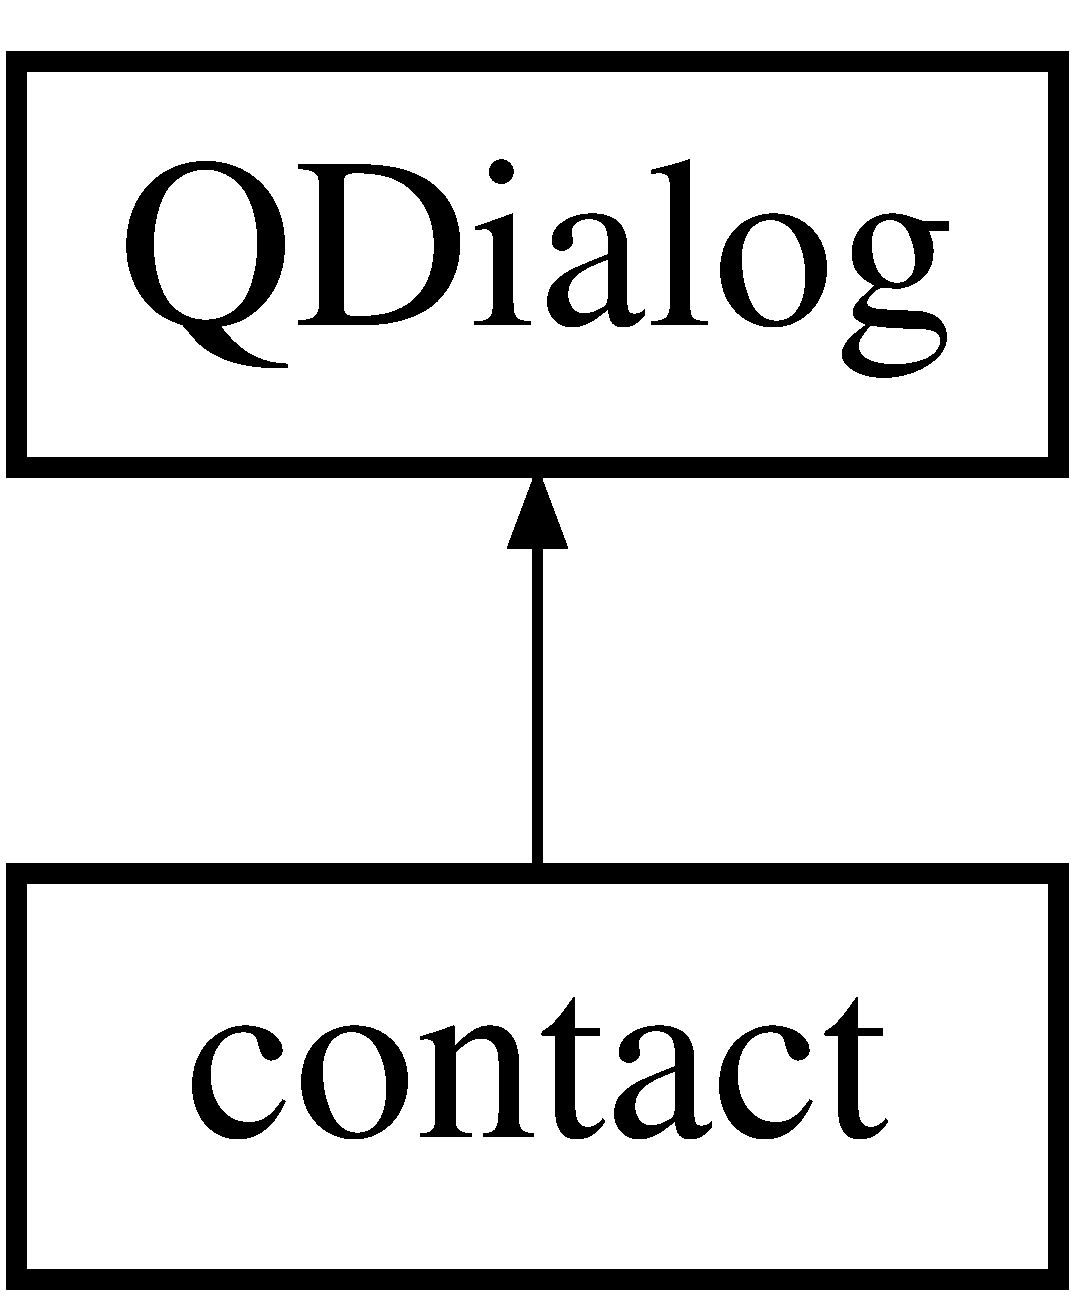
\includegraphics[height=2.000000cm]{classcontact}
\end{center}
\end{figure}
\subsection*{Public Member Functions}
\begin{DoxyCompactItemize}
\item 
\mbox{\Hypertarget{classcontact_a530a040af99efa8cb80a0e97fbd1bf34}\label{classcontact_a530a040af99efa8cb80a0e97fbd1bf34}} 
{\bfseries contact} (Q\+Widget $\ast$parent=0)
\end{DoxyCompactItemize}


The documentation for this class was generated from the following files\+:\begin{DoxyCompactItemize}
\item 
contact.\+h\item 
contact.\+cpp\end{DoxyCompactItemize}

\hypertarget{class_ellipse}{}\section{Ellipse Class Reference}
\label{class_ellipse}\index{Ellipse@{Ellipse}}
Inheritance diagram for Ellipse\+:\begin{figure}[H]
\begin{center}
\leavevmode
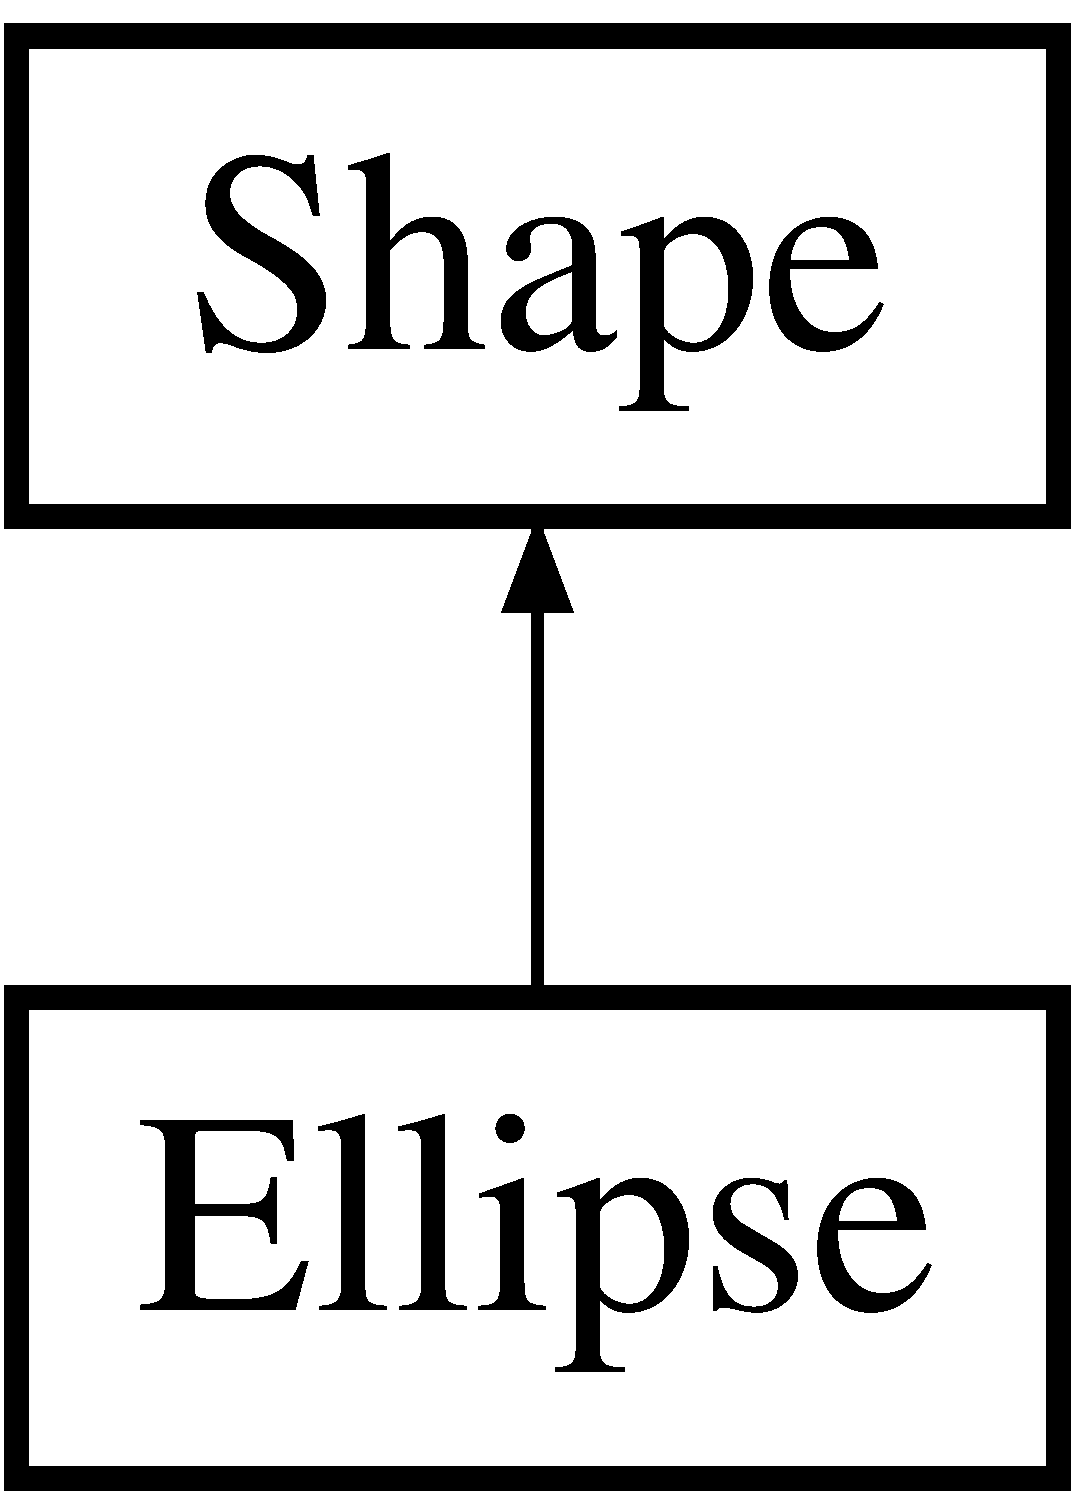
\includegraphics[height=2.000000cm]{class_ellipse}
\end{center}
\end{figure}
\subsection*{Public Member Functions}
\begin{DoxyCompactItemize}
\item 
\mbox{\Hypertarget{class_ellipse_a312c0cf0e855dc79d37c07ec52bf202e}\label{class_ellipse_a312c0cf0e855dc79d37c07ec52bf202e}} 
void {\bfseries draw} ()
\item 
\mbox{\Hypertarget{class_ellipse_a143b160178dd490a441ae0aa2ebd1312}\label{class_ellipse_a143b160178dd490a441ae0aa2ebd1312}} 
void {\bfseries move} ()
\item 
\mbox{\Hypertarget{class_ellipse_a6d732cab362846f9a796d84af2031c37}\label{class_ellipse_a6d732cab362846f9a796d84af2031c37}} 
int {\bfseries get\+Perimeter} ()
\item 
\mbox{\Hypertarget{class_ellipse_a8099b7e5018cf1de2ac2b4d08782a5e5}\label{class_ellipse_a8099b7e5018cf1de2ac2b4d08782a5e5}} 
int {\bfseries get\+Area} ()
\item 
\mbox{\Hypertarget{class_ellipse_a7a785026c16fcdfec458dd4c63f69241}\label{class_ellipse_a7a785026c16fcdfec458dd4c63f69241}} 
Q\+Pen {\bfseries get\+Pen} ()
\item 
\mbox{\Hypertarget{class_ellipse_a362fdff0cc4fe3fe4a06febc6f71cccc}\label{class_ellipse_a362fdff0cc4fe3fe4a06febc6f71cccc}} 
Q\+Brush {\bfseries get\+Brush} ()
\item 
\mbox{\Hypertarget{class_ellipse_aee29fe26c64567b068a4c5b10824ab5c}\label{class_ellipse_aee29fe26c64567b068a4c5b10824ab5c}} 
{\bfseries Ellipse} (int a1, int b1)
\item 
\mbox{\Hypertarget{class_ellipse_a425c228f8845bb684601f69812775b62}\label{class_ellipse_a425c228f8845bb684601f69812775b62}} 
{\bfseries Ellipse} (const \mbox{\hyperlink{class_ellipse}{Ellipse}} \&other)
\item 
\mbox{\Hypertarget{class_ellipse_a6735ab5f8302ab49001b5d5fa18e69c1}\label{class_ellipse_a6735ab5f8302ab49001b5d5fa18e69c1}} 
void {\bfseries get\+Data} ()
\end{DoxyCompactItemize}
\subsection*{Additional Inherited Members}


The documentation for this class was generated from the following file\+:\begin{DoxyCompactItemize}
\item 
ellipse.\+h\end{DoxyCompactItemize}

\hypertarget{class_line}{}\section{Line Class Reference}
\label{class_line}\index{Line@{Line}}
Inheritance diagram for Line\+:\begin{figure}[H]
\begin{center}
\leavevmode
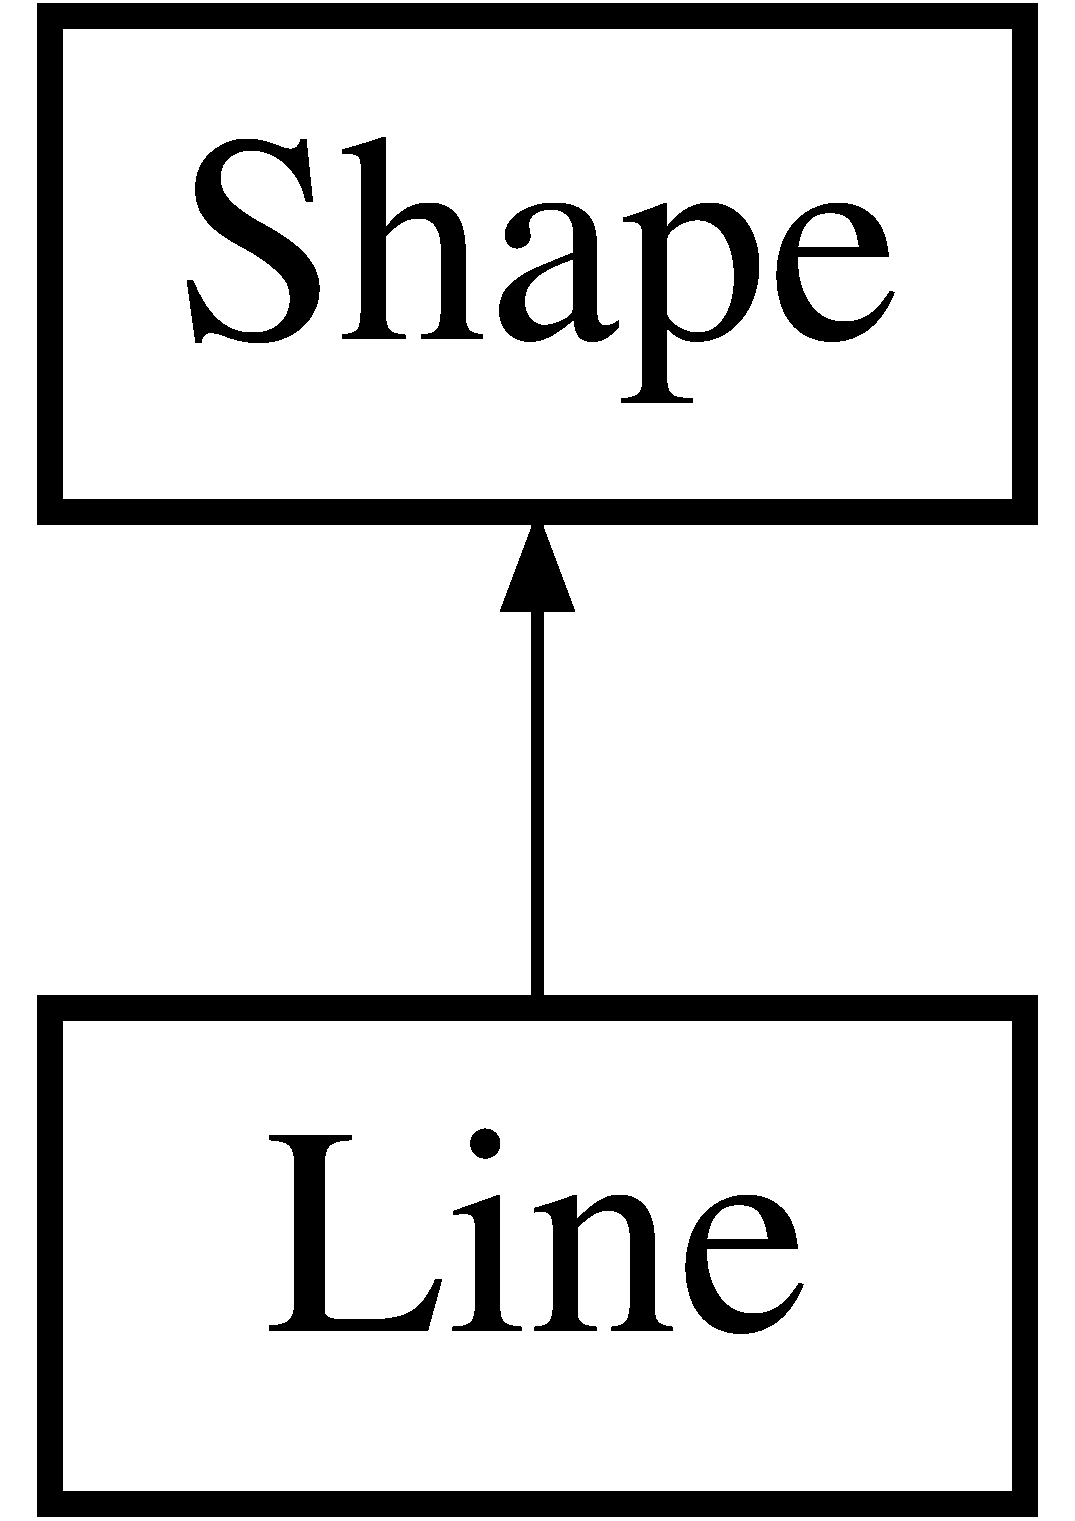
\includegraphics[height=2.000000cm]{class_line}
\end{center}
\end{figure}
\subsection*{Public Member Functions}
\begin{DoxyCompactItemize}
\item 
\mbox{\Hypertarget{class_line_ab6265993bf5acbc28830181c3e712f10}\label{class_line_ab6265993bf5acbc28830181c3e712f10}} 
void {\bfseries draw} ()
\item 
\mbox{\Hypertarget{class_line_a2795de3dd5a6eb05a1b8aaec57aa1f9f}\label{class_line_a2795de3dd5a6eb05a1b8aaec57aa1f9f}} 
void {\bfseries move} ()
\item 
\mbox{\Hypertarget{class_line_a34ff8a27e7c17a4d4cbc50ddd8769312}\label{class_line_a34ff8a27e7c17a4d4cbc50ddd8769312}} 
int {\bfseries get\+Perimeter} ()
\item 
\mbox{\Hypertarget{class_line_ab66fd39f66f4caa5284f0e9c2d3a36fa}\label{class_line_ab66fd39f66f4caa5284f0e9c2d3a36fa}} 
int {\bfseries get\+Area} ()
\item 
\mbox{\Hypertarget{class_line_a5f45efd96d106724b175d8d52549b446}\label{class_line_a5f45efd96d106724b175d8d52549b446}} 
Q\+Pen {\bfseries get\+Pen} ()
\item 
\mbox{\Hypertarget{class_line_a8ca597644c62d0b8ab63bfaaab1dc494}\label{class_line_a8ca597644c62d0b8ab63bfaaab1dc494}} 
{\bfseries Line} (int a1, int b1, int a2, int b2)
\item 
\mbox{\Hypertarget{class_line_ac40968264c0af3b70506c13ce3b70b5b}\label{class_line_ac40968264c0af3b70506c13ce3b70b5b}} 
{\bfseries Line} (const \mbox{\hyperlink{class_line}{Line}} \&other)
\end{DoxyCompactItemize}
\subsection*{Additional Inherited Members}


The documentation for this class was generated from the following file\+:\begin{DoxyCompactItemize}
\item 
line.\+h\end{DoxyCompactItemize}

\hypertarget{classlog_in}{}\section{log\+In Class Reference}
\label{classlog_in}\index{log\+In@{log\+In}}
Inheritance diagram for log\+In\+:\begin{figure}[H]
\begin{center}
\leavevmode
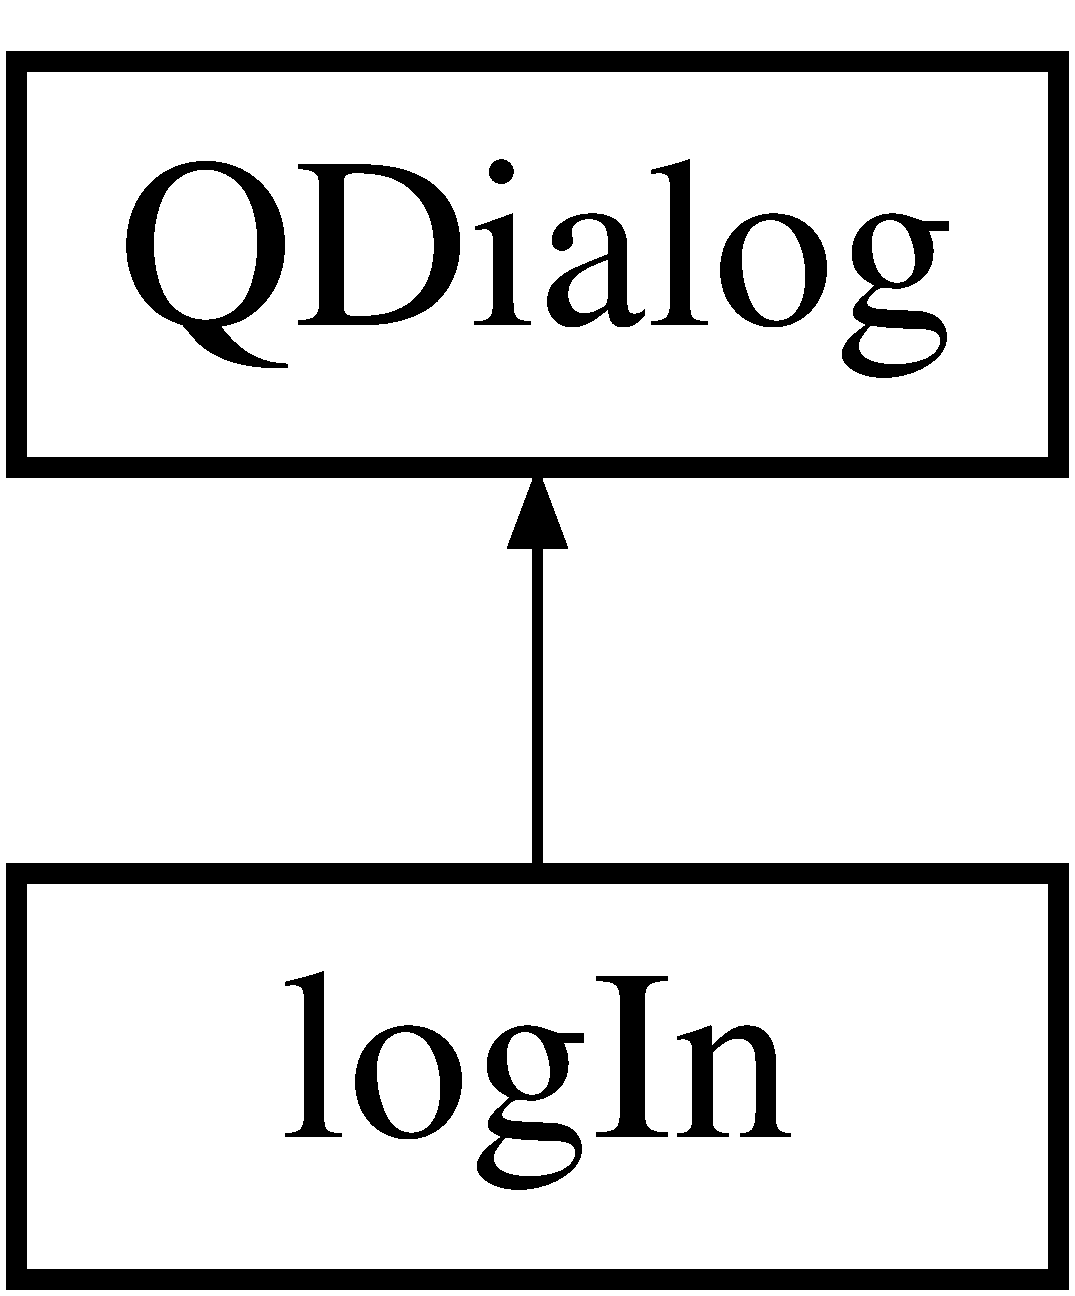
\includegraphics[height=2.000000cm]{classlog_in}
\end{center}
\end{figure}
\subsection*{Public Member Functions}
\begin{DoxyCompactItemize}
\item 
\mbox{\Hypertarget{classlog_in_ab9ea8b8e3ab32fe2acdc5058b5ba078f}\label{classlog_in_ab9ea8b8e3ab32fe2acdc5058b5ba078f}} 
{\bfseries log\+In} (Q\+Widget $\ast$parent=0)
\end{DoxyCompactItemize}


The documentation for this class was generated from the following files\+:\begin{DoxyCompactItemize}
\item 
login.\+h\item 
login.\+cpp\end{DoxyCompactItemize}

\hypertarget{class_main_window}{}\section{Main\+Window Class Reference}
\label{class_main_window}\index{Main\+Window@{Main\+Window}}
Inheritance diagram for Main\+Window\+:\begin{figure}[H]
\begin{center}
\leavevmode
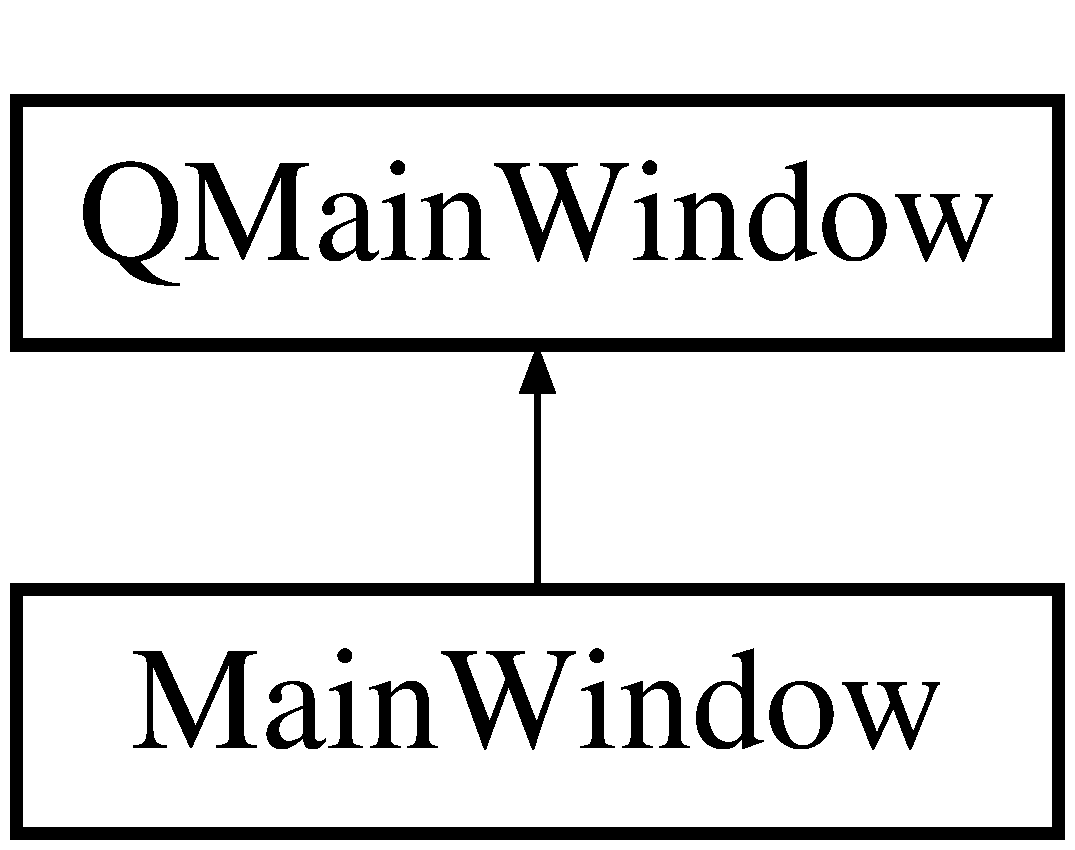
\includegraphics[height=2.000000cm]{class_main_window}
\end{center}
\end{figure}
\subsection*{Public Member Functions}
\begin{DoxyCompactItemize}
\item 
\mbox{\Hypertarget{class_main_window_a996c5a2b6f77944776856f08ec30858d}\label{class_main_window_a996c5a2b6f77944776856f08ec30858d}} 
{\bfseries Main\+Window} (Q\+Widget $\ast$parent=nullptr)
\end{DoxyCompactItemize}


The documentation for this class was generated from the following files\+:\begin{DoxyCompactItemize}
\item 
mainwindow.\+h\item 
mainwindow.\+cpp\end{DoxyCompactItemize}

\hypertarget{class_polygon}{}\section{Polygon Class Reference}
\label{class_polygon}\index{Polygon@{Polygon}}
Inheritance diagram for Polygon\+:\begin{figure}[H]
\begin{center}
\leavevmode
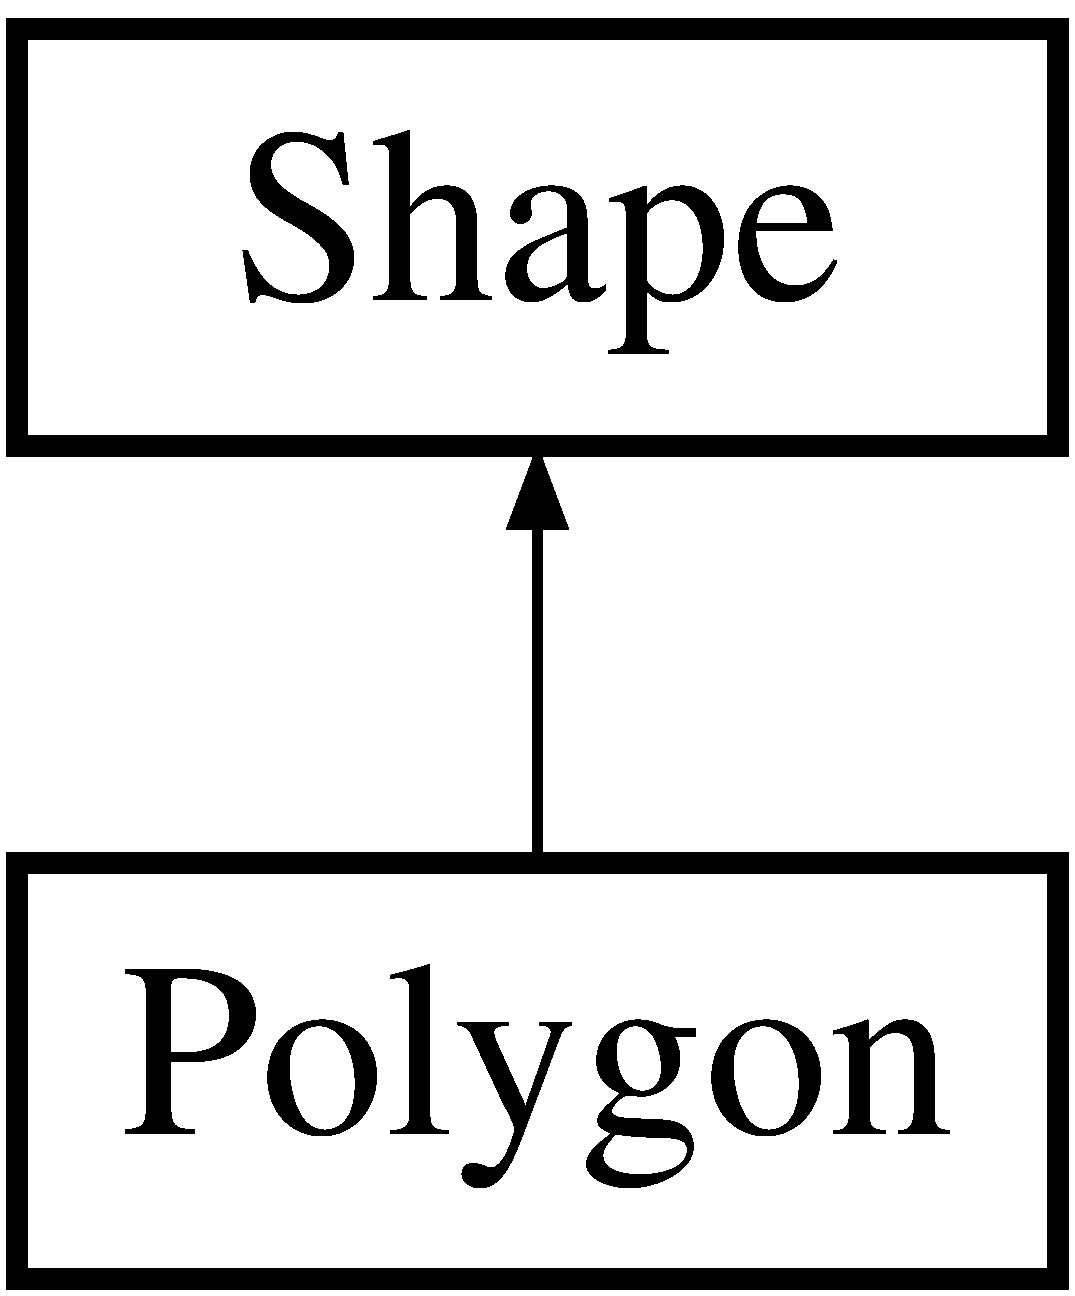
\includegraphics[height=2.000000cm]{class_polygon}
\end{center}
\end{figure}
\subsection*{Public Member Functions}
\begin{DoxyCompactItemize}
\item 
\mbox{\Hypertarget{class_polygon_a17428a7d7dff4653c905b91020a9f803}\label{class_polygon_a17428a7d7dff4653c905b91020a9f803}} 
void {\bfseries draw} ()
\item 
\mbox{\Hypertarget{class_polygon_ad2931f86bb11263a87027b4ea9002e98}\label{class_polygon_ad2931f86bb11263a87027b4ea9002e98}} 
void {\bfseries move} ()
\item 
\mbox{\Hypertarget{class_polygon_a134c393d322723057d62e2ad85c73885}\label{class_polygon_a134c393d322723057d62e2ad85c73885}} 
int {\bfseries get\+Perimeter} ()
\item 
\mbox{\Hypertarget{class_polygon_a392d9f070fee280614eaa5b702d06537}\label{class_polygon_a392d9f070fee280614eaa5b702d06537}} 
int {\bfseries get\+Area} ()
\item 
\mbox{\Hypertarget{class_polygon_a398faa5ff795637a7a02b8bc78b40356}\label{class_polygon_a398faa5ff795637a7a02b8bc78b40356}} 
Q\+Pen {\bfseries get\+Pen} ()
\item 
\mbox{\Hypertarget{class_polygon_af10e35bb2d7eb19c471b501e733fda5a}\label{class_polygon_af10e35bb2d7eb19c471b501e733fda5a}} 
Q\+Brush {\bfseries get\+Brush} ()
\item 
\mbox{\Hypertarget{class_polygon_a2a6e9a2acc12944ad2e70c61d3479efa}\label{class_polygon_a2a6e9a2acc12944ad2e70c61d3479efa}} 
Q\+Point $\ast$ {\bfseries get\+Points} ()
\end{DoxyCompactItemize}
\subsection*{Additional Inherited Members}


The documentation for this class was generated from the following file\+:\begin{DoxyCompactItemize}
\item 
polygon.\+h\end{DoxyCompactItemize}

\hypertarget{class_polyline}{}\section{Polyline Class Reference}
\label{class_polyline}\index{Polyline@{Polyline}}
Inheritance diagram for Polyline\+:\begin{figure}[H]
\begin{center}
\leavevmode
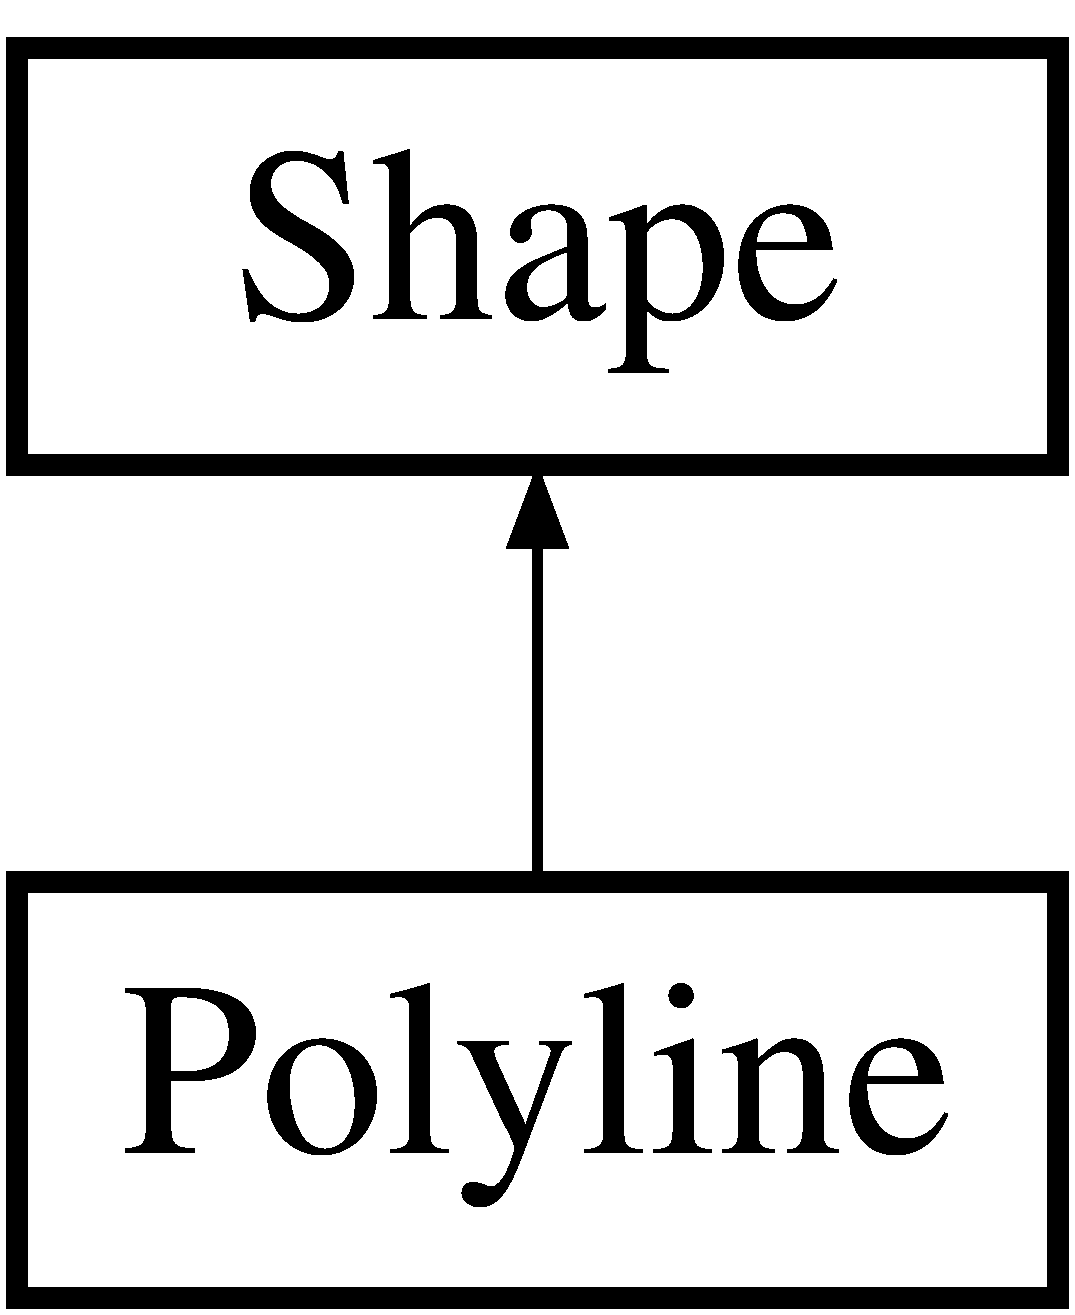
\includegraphics[height=2.000000cm]{class_polyline}
\end{center}
\end{figure}
\subsection*{Public Member Functions}
\begin{DoxyCompactItemize}
\item 
\mbox{\Hypertarget{class_polyline_a21ea8147cb2a0d8d9b61af7b62520395}\label{class_polyline_a21ea8147cb2a0d8d9b61af7b62520395}} 
void {\bfseries draw} ()
\item 
\mbox{\Hypertarget{class_polyline_a6a94f8224305b0a63425ab434cf70c33}\label{class_polyline_a6a94f8224305b0a63425ab434cf70c33}} 
void {\bfseries move} ()
\item 
\mbox{\Hypertarget{class_polyline_a330517ebe729fea9157474f169c8f412}\label{class_polyline_a330517ebe729fea9157474f169c8f412}} 
int {\bfseries get\+Perimeter} ()
\item 
\mbox{\Hypertarget{class_polyline_aac434c98a3e3e11ca89d605fe1b7e469}\label{class_polyline_aac434c98a3e3e11ca89d605fe1b7e469}} 
int {\bfseries get\+Area} ()
\item 
\mbox{\Hypertarget{class_polyline_a02e173040039bad2dabc022f73957091}\label{class_polyline_a02e173040039bad2dabc022f73957091}} 
Q\+Pen {\bfseries get\+Pen} ()
\item 
\mbox{\Hypertarget{class_polyline_a08321eef3c83d6b3ee8d9dab29f6aaf9}\label{class_polyline_a08321eef3c83d6b3ee8d9dab29f6aaf9}} 
Q\+Point $\ast$ {\bfseries get\+Points} ()
\end{DoxyCompactItemize}
\subsection*{Additional Inherited Members}


The documentation for this class was generated from the following file\+:\begin{DoxyCompactItemize}
\item 
polyline.\+h\end{DoxyCompactItemize}

\hypertarget{class_rectangle}{}\section{Rectangle Class Reference}
\label{class_rectangle}\index{Rectangle@{Rectangle}}
Inheritance diagram for Rectangle\+:\begin{figure}[H]
\begin{center}
\leavevmode
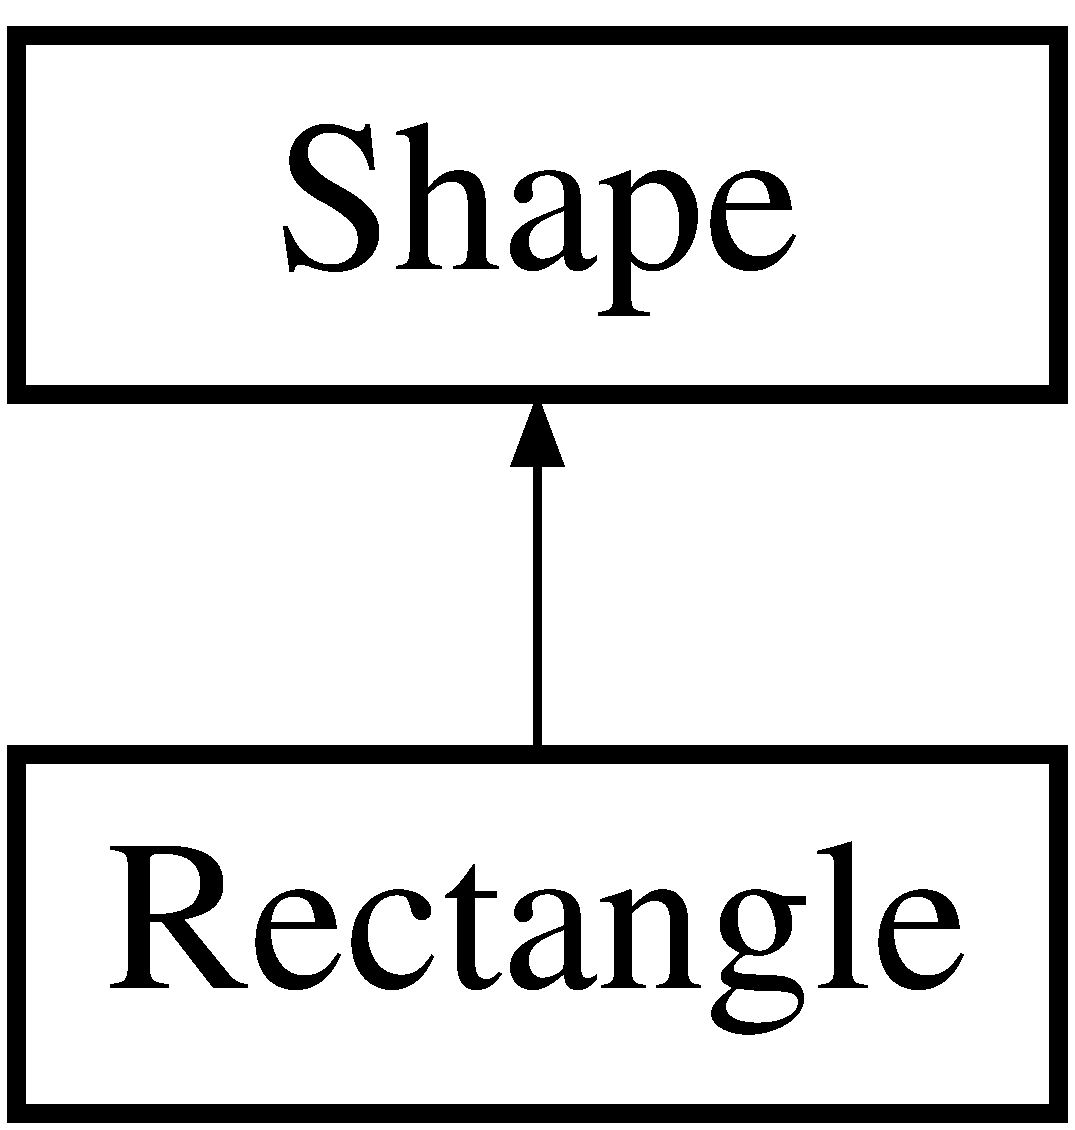
\includegraphics[height=2.000000cm]{class_rectangle}
\end{center}
\end{figure}
\subsection*{Public Member Functions}
\begin{DoxyCompactItemize}
\item 
\mbox{\Hypertarget{class_rectangle_ac895c67f1d6337e3b4f72663b17dd299}\label{class_rectangle_ac895c67f1d6337e3b4f72663b17dd299}} 
void {\bfseries draw} ()
\item 
\mbox{\Hypertarget{class_rectangle_ac22f117344cc27842d78465573ade090}\label{class_rectangle_ac22f117344cc27842d78465573ade090}} 
void {\bfseries move} ()
\item 
\mbox{\Hypertarget{class_rectangle_a59cc981af638e29c752eb38d470eb0dc}\label{class_rectangle_a59cc981af638e29c752eb38d470eb0dc}} 
int {\bfseries get\+Perimeter} ()
\item 
\mbox{\Hypertarget{class_rectangle_a5d7633ce9d9bd356f0a8ce1eb5b4b2ae}\label{class_rectangle_a5d7633ce9d9bd356f0a8ce1eb5b4b2ae}} 
int {\bfseries get\+Area} ()
\item 
\mbox{\Hypertarget{class_rectangle_af81f6576c829b41bfe0b7852931a7107}\label{class_rectangle_af81f6576c829b41bfe0b7852931a7107}} 
Q\+Pen {\bfseries get\+Pen} ()
\item 
\mbox{\Hypertarget{class_rectangle_a6f328f3878366ba97f845eca63f9f2c0}\label{class_rectangle_a6f328f3878366ba97f845eca63f9f2c0}} 
Q\+Brush {\bfseries get\+Brush} ()
\item 
\mbox{\Hypertarget{class_rectangle_af0c06d1e26a2a296b380fcf0e157d78e}\label{class_rectangle_af0c06d1e26a2a296b380fcf0e157d78e}} 
Q\+Rect {\bfseries get\+Rect} ()
\item 
\mbox{\Hypertarget{class_rectangle_a14bebb658c850ef730fb3e65adab1f91}\label{class_rectangle_a14bebb658c850ef730fb3e65adab1f91}} 
{\bfseries Rectangle} (\mbox{\hyperlink{class_rectangle}{Rectangle}} \&other)
\item 
\mbox{\Hypertarget{class_rectangle_ac2bb13ef1af8fe288bf46c92e95fb875}\label{class_rectangle_ac2bb13ef1af8fe288bf46c92e95fb875}} 
{\bfseries Rectangle} (int length, int width)
\end{DoxyCompactItemize}
\subsection*{Additional Inherited Members}


The documentation for this class was generated from the following file\+:\begin{DoxyCompactItemize}
\item 
rectangle.\+h\end{DoxyCompactItemize}

\hypertarget{class_render_area}{}\section{Render\+Area Class Reference}
\label{class_render_area}\index{Render\+Area@{Render\+Area}}
Inheritance diagram for Render\+Area\+:\begin{figure}[H]
\begin{center}
\leavevmode
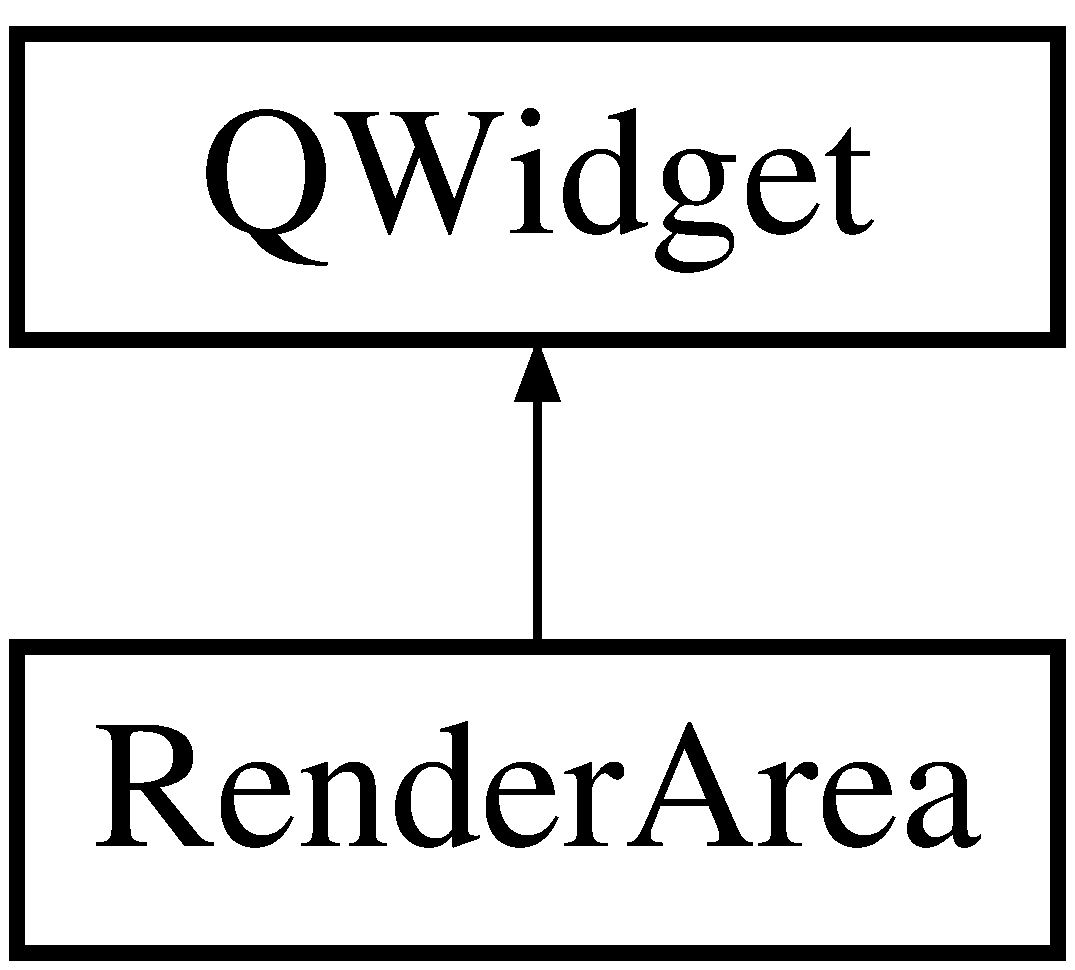
\includegraphics[height=2.000000cm]{class_render_area}
\end{center}
\end{figure}
\subsection*{Public Types}
\begin{DoxyCompactItemize}
\item 
\mbox{\Hypertarget{class_render_area_a45c0e3befbec666b5f7ae3beeffc9b80}\label{class_render_area_a45c0e3befbec666b5f7ae3beeffc9b80}} 
enum {\bfseries Shapes} \{ \newline
{\bfseries LineE}, 
{\bfseries PolylineE}, 
{\bfseries RectangleE}, 
{\bfseries EllipseE}, 
\newline
{\bfseries PolygonE}, 
{\bfseries TextE}
 \}
\end{DoxyCompactItemize}
\subsection*{Public Slots}
\begin{DoxyCompactItemize}
\item 
\mbox{\Hypertarget{class_render_area_a7b0482d994c6631cd74a32a88c50a94e}\label{class_render_area_a7b0482d994c6631cd74a32a88c50a94e}} 
void {\bfseries set\+Shape} (Shapes shape)
\item 
\mbox{\Hypertarget{class_render_area_a209db7987984687b05ee02e6784ad782}\label{class_render_area_a209db7987984687b05ee02e6784ad782}} 
void {\bfseries set\+Pen} (const Q\+Pen \&pen)
\item 
\mbox{\Hypertarget{class_render_area_a89dbd44a79ba820ae8d651f30abc56b1}\label{class_render_area_a89dbd44a79ba820ae8d651f30abc56b1}} 
void {\bfseries set\+Brush} (const Q\+Brush \&brush)
\item 
\mbox{\Hypertarget{class_render_area_afe6c01e6f89bef67a2322c8245efb134}\label{class_render_area_afe6c01e6f89bef67a2322c8245efb134}} 
void {\bfseries set\+Transformed} (bool transformed)
\end{DoxyCompactItemize}
\subsection*{Public Member Functions}
\begin{DoxyCompactItemize}
\item 
\mbox{\Hypertarget{class_render_area_a2e337a64fb1f619e6c63832bd1027f99}\label{class_render_area_a2e337a64fb1f619e6c63832bd1027f99}} 
{\bfseries Render\+Area} (Q\+Widget $\ast$parent=0)
\item 
\mbox{\Hypertarget{class_render_area_a9df5bc259ad4238f208bfd4657b9afab}\label{class_render_area_a9df5bc259ad4238f208bfd4657b9afab}} 
Q\+Size {\bfseries minimum\+Size\+Hint} () const Q\+\_\+\+D\+E\+C\+L\+\_\+\+O\+V\+E\+R\+R\+I\+DE
\item 
\mbox{\Hypertarget{class_render_area_a3c8c7860b578b7b0114656383c69f149}\label{class_render_area_a3c8c7860b578b7b0114656383c69f149}} 
Q\+Size {\bfseries size\+Hint} () const Q\+\_\+\+D\+E\+C\+L\+\_\+\+O\+V\+E\+R\+R\+I\+DE
\end{DoxyCompactItemize}
\subsection*{Protected Member Functions}
\begin{DoxyCompactItemize}
\item 
\mbox{\Hypertarget{class_render_area_ac7463f6acc32ec6a1e6e494e19297892}\label{class_render_area_ac7463f6acc32ec6a1e6e494e19297892}} 
void {\bfseries paint\+Event} (Q\+Paint\+Event $\ast$event) Q\+\_\+\+D\+E\+C\+L\+\_\+\+O\+V\+E\+R\+R\+I\+DE
\end{DoxyCompactItemize}


The documentation for this class was generated from the following files\+:\begin{DoxyCompactItemize}
\item 
renderarea.\+h\item 
renderarea.\+cpp\end{DoxyCompactItemize}

\hypertarget{class_shape}{}\section{Shape Class Reference}
\label{class_shape}\index{Shape@{Shape}}
Inheritance diagram for Shape\+:\begin{figure}[H]
\begin{center}
\leavevmode
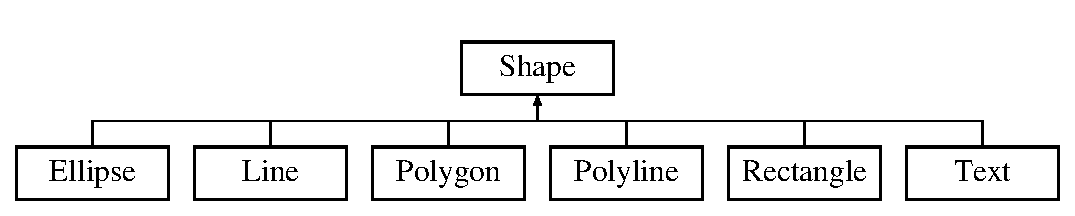
\includegraphics[height=2.000000cm]{class_shape}
\end{center}
\end{figure}
\subsection*{Public Member Functions}
\begin{DoxyCompactItemize}
\item 
\mbox{\Hypertarget{class_shape_a058f2fada39a73f6640f15a0ac715ba9}\label{class_shape_a058f2fada39a73f6640f15a0ac715ba9}} 
{\bfseries Shape} (int id)
\item 
\mbox{\Hypertarget{class_shape_a5d5b669bf375fd84f66c47936649cae6}\label{class_shape_a5d5b669bf375fd84f66c47936649cae6}} 
{\bfseries Shape} (int id, Qt\+::\+Global\+Color penC, int penW, Qt\+::\+Pen\+Style penS, Qt\+::\+Pen\+Cap\+Style capS, Qt\+::\+Pen\+Join\+Style joinS)
\item 
\mbox{\Hypertarget{class_shape_aa6c604f5b5836cf4f754e823e20aaac6}\label{class_shape_aa6c604f5b5836cf4f754e823e20aaac6}} 
{\bfseries Shape} (int id, Qt\+::\+Global\+Color penC, int penW, Qt\+::\+Pen\+Style penS, Qt\+::\+Pen\+Cap\+Style capS, Qt\+::\+Pen\+Join\+Style joinS, Qt\+::\+Global\+Color brushC, Qt\+::\+Brush\+Style brushS)
\item 
\mbox{\Hypertarget{class_shape_ad24c5659cb3bdbeb8881b62a8402df98}\label{class_shape_ad24c5659cb3bdbeb8881b62a8402df98}} 
int {\bfseries get\+Id} ()
\item 
\mbox{\Hypertarget{class_shape_afacc5aad8e37308c3ce8fef768199b05}\label{class_shape_afacc5aad8e37308c3ce8fef768199b05}} 
virtual void {\bfseries draw} ()=0
\item 
\mbox{\Hypertarget{class_shape_a7e615d857e9ff5f1ad28a04bcd5d4e79}\label{class_shape_a7e615d857e9ff5f1ad28a04bcd5d4e79}} 
virtual void {\bfseries move} ()=0
\item 
\mbox{\Hypertarget{class_shape_a5c48c218574bbdd03cee949b0375820a}\label{class_shape_a5c48c218574bbdd03cee949b0375820a}} 
virtual int {\bfseries get\+Perimeter} ()=0
\item 
\mbox{\Hypertarget{class_shape_a04eb100a2d610e742f9f60f88e18fa12}\label{class_shape_a04eb100a2d610e742f9f60f88e18fa12}} 
virtual int {\bfseries get\+Area} ()=0
\item 
\mbox{\Hypertarget{class_shape_ad63168173d9f946230ca75277807163d}\label{class_shape_ad63168173d9f946230ca75277807163d}} 
bool {\bfseries operator==} (const \mbox{\hyperlink{class_shape}{Shape}} \&shape2)
\item 
\mbox{\Hypertarget{class_shape_aea09877f437758ffe34b2414c17b826d}\label{class_shape_aea09877f437758ffe34b2414c17b826d}} 
bool {\bfseries operator$<$=} (const \mbox{\hyperlink{class_shape}{Shape}} \&shape2)
\item 
\mbox{\Hypertarget{class_shape_a33d41873210e01fc1681dda1484d614f}\label{class_shape_a33d41873210e01fc1681dda1484d614f}} 
{\bfseries Shape} (const \mbox{\hyperlink{class_shape}{Shape}} \&)
\end{DoxyCompactItemize}
\subsection*{Protected Attributes}
\begin{DoxyCompactItemize}
\item 
\mbox{\Hypertarget{class_shape_a54468486d6f4b88380a4ca0c5cf3c978}\label{class_shape_a54468486d6f4b88380a4ca0c5cf3c978}} 
Qt\+::\+Global\+Color {\bfseries pen\+Color}
\item 
\mbox{\Hypertarget{class_shape_aeb1f782a11b840f138392c64ad53d11e}\label{class_shape_aeb1f782a11b840f138392c64ad53d11e}} 
int {\bfseries pen\+Width}
\item 
\mbox{\Hypertarget{class_shape_a0ca3168a8b628b6172c8d7c2050bd0b2}\label{class_shape_a0ca3168a8b628b6172c8d7c2050bd0b2}} 
Qt\+::\+Pen\+Style {\bfseries pen\+Style}
\item 
\mbox{\Hypertarget{class_shape_ab49a905e221eae2ba352d1ebf0b0c6b7}\label{class_shape_ab49a905e221eae2ba352d1ebf0b0c6b7}} 
Qt\+::\+Pen\+Cap\+Style {\bfseries cap\+Style}
\item 
\mbox{\Hypertarget{class_shape_a97bb96c2a982a416c5c522b692209318}\label{class_shape_a97bb96c2a982a416c5c522b692209318}} 
Qt\+::\+Pen\+Join\+Style {\bfseries join\+Style}
\item 
\mbox{\Hypertarget{class_shape_a705f872905fc3f23f059f57051af79c6}\label{class_shape_a705f872905fc3f23f059f57051af79c6}} 
Qt\+::\+Global\+Color {\bfseries brush\+Color}
\item 
\mbox{\Hypertarget{class_shape_a6eeb8fdef70508b76558c2bf95f19360}\label{class_shape_a6eeb8fdef70508b76558c2bf95f19360}} 
Qt\+::\+Brush\+Style {\bfseries brush\+Style}
\item 
\mbox{\Hypertarget{class_shape_a761a117dfc4b157944e512b8a4c89fde}\label{class_shape_a761a117dfc4b157944e512b8a4c89fde}} 
Q\+Painter {\bfseries painter}
\end{DoxyCompactItemize}


The documentation for this class was generated from the following file\+:\begin{DoxyCompactItemize}
\item 
shape.\+h\end{DoxyCompactItemize}

\hypertarget{class_text}{}\section{Text Class Reference}
\label{class_text}\index{Text@{Text}}
Inheritance diagram for Text\+:\begin{figure}[H]
\begin{center}
\leavevmode
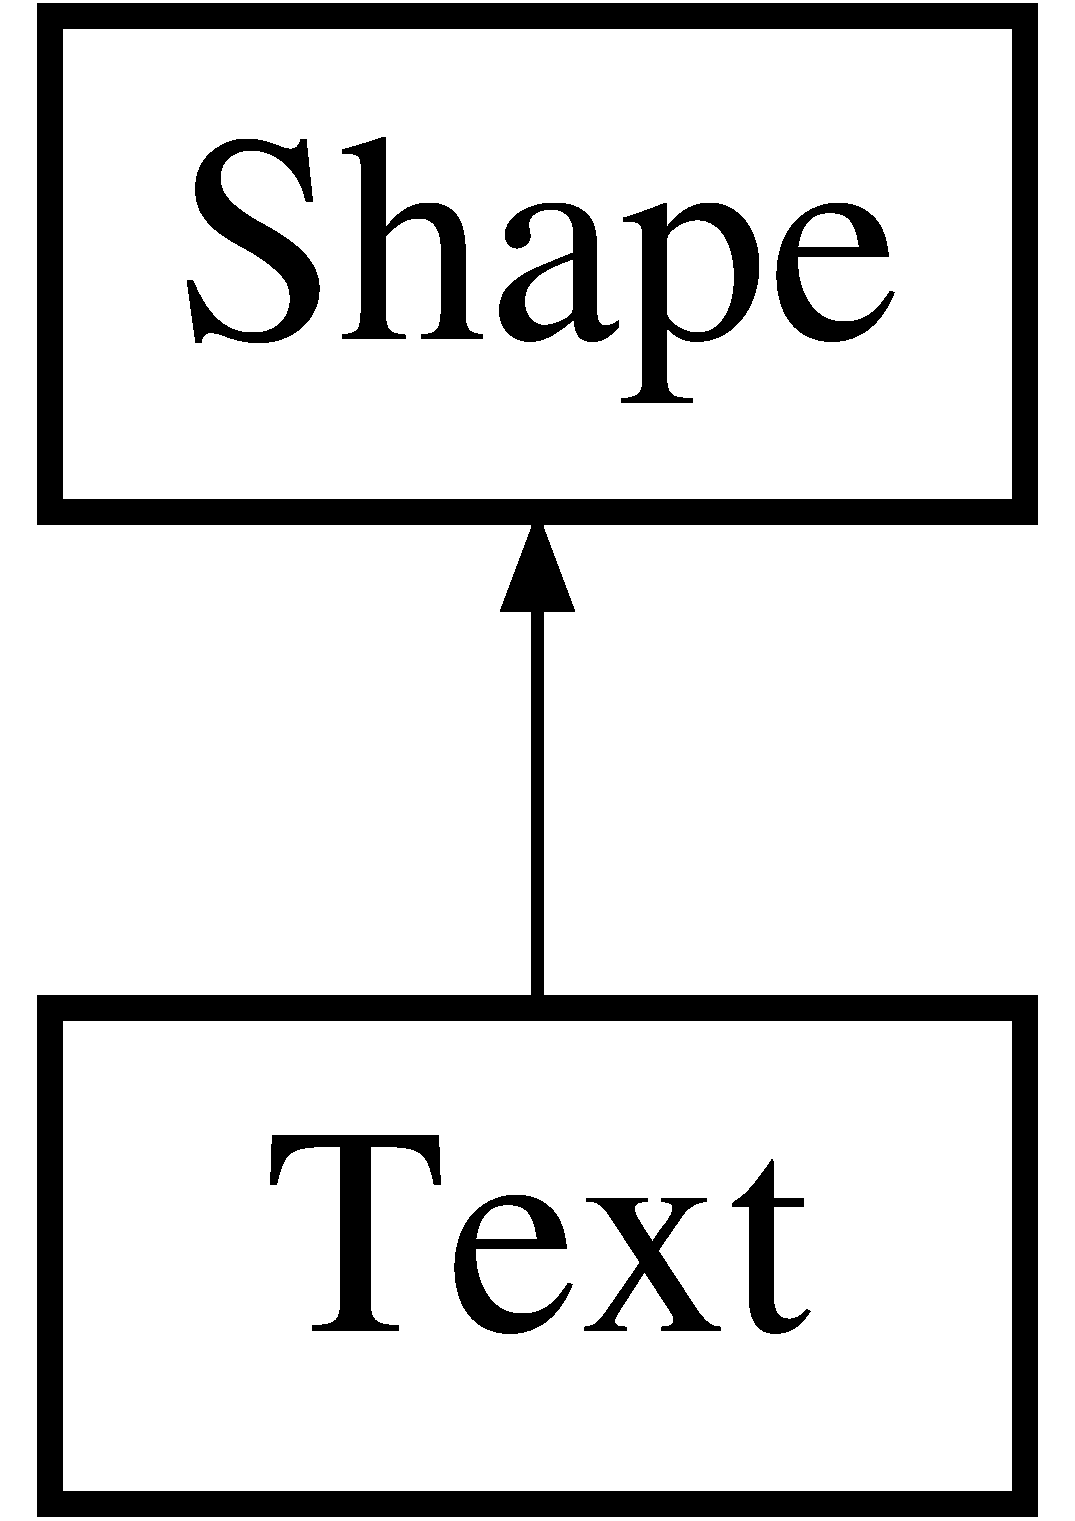
\includegraphics[height=2.000000cm]{class_text}
\end{center}
\end{figure}
\subsection*{Public Member Functions}
\begin{DoxyCompactItemize}
\item 
\mbox{\Hypertarget{class_text_adedc069a9ad622bf9d2cf6d194a01b39}\label{class_text_adedc069a9ad622bf9d2cf6d194a01b39}} 
void {\bfseries draw} ()
\item 
\mbox{\Hypertarget{class_text_afb3b7b69bd321c09e8bfbdebb6d21e11}\label{class_text_afb3b7b69bd321c09e8bfbdebb6d21e11}} 
void {\bfseries move} ()
\item 
\mbox{\Hypertarget{class_text_a77461345a606fb745f3ee30977c89031}\label{class_text_a77461345a606fb745f3ee30977c89031}} 
int {\bfseries get\+Perimeter} ()
\item 
\mbox{\Hypertarget{class_text_a4be6e639837d756d7d346ab785a5f04e}\label{class_text_a4be6e639837d756d7d346ab785a5f04e}} 
int {\bfseries get\+Area} ()
\item 
\mbox{\Hypertarget{class_text_a81d3c6b7ab019dd8eed8b389007152fa}\label{class_text_a81d3c6b7ab019dd8eed8b389007152fa}} 
Q\+Rect {\bfseries get\+Rect} ()
\item 
\mbox{\Hypertarget{class_text_a63ccf2f936b2230e2a980eaf875509a2}\label{class_text_a63ccf2f936b2230e2a980eaf875509a2}} 
Qt\+::\+Alignment {\bfseries get\+Align} ()
\item 
\mbox{\Hypertarget{class_text_a2da9d282ef7497a76d3edf04b64ce39c}\label{class_text_a2da9d282ef7497a76d3edf04b64ce39c}} 
string {\bfseries get\+String} ()
\end{DoxyCompactItemize}
\subsection*{Additional Inherited Members}


The documentation for this class was generated from the following file\+:\begin{DoxyCompactItemize}
\item 
text.\+h\end{DoxyCompactItemize}

\hypertarget{class_window}{}\section{Window Class Reference}
\label{class_window}\index{Window@{Window}}
Inheritance diagram for Window\+:\begin{figure}[H]
\begin{center}
\leavevmode
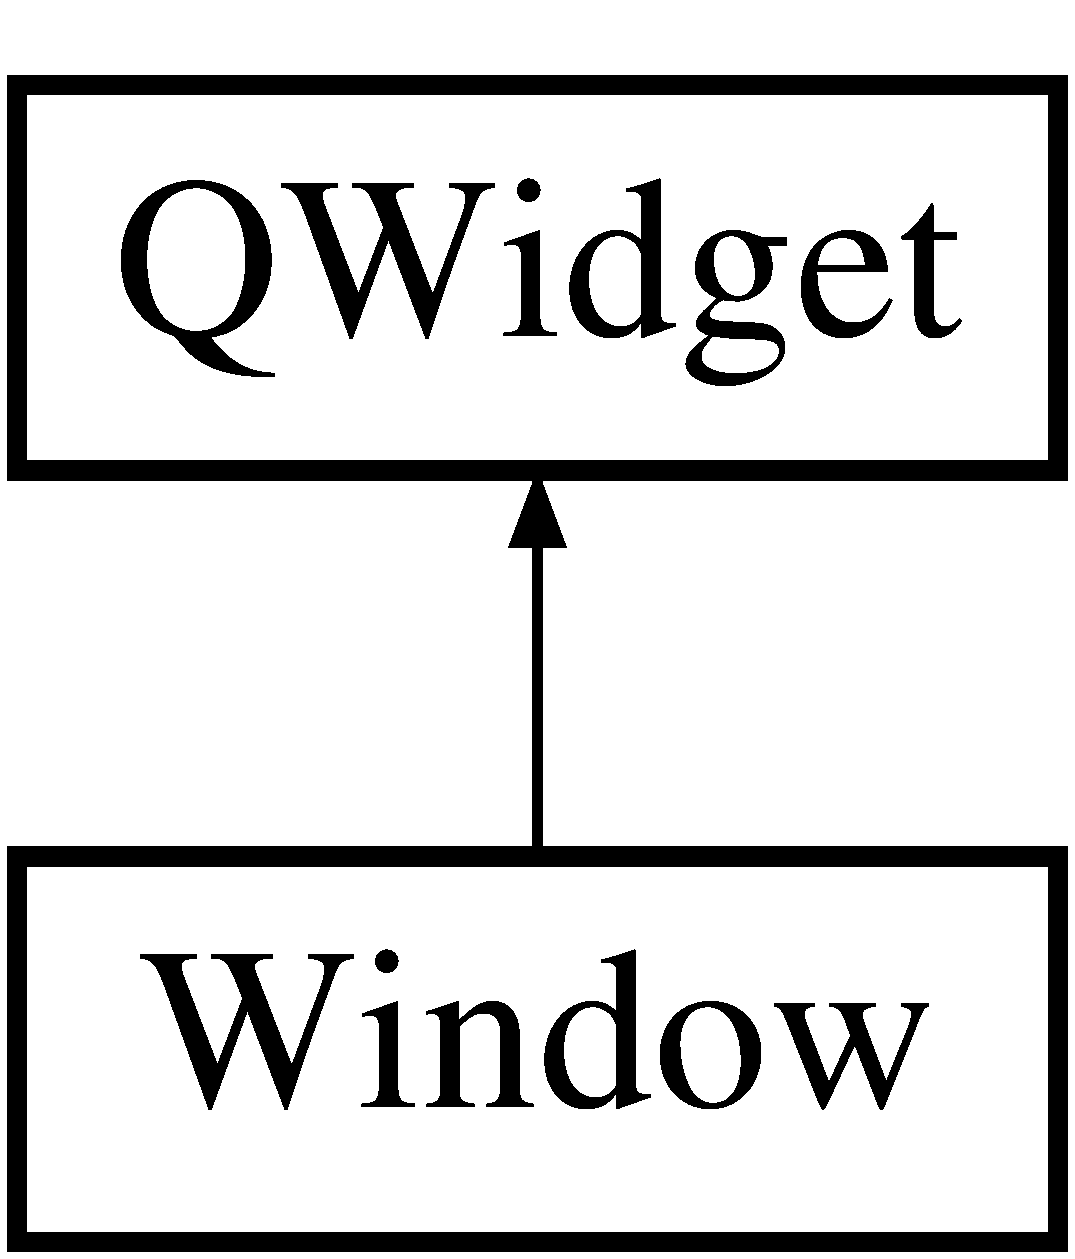
\includegraphics[height=2.000000cm]{class_window}
\end{center}
\end{figure}
\subsection*{Public Member Functions}
\begin{DoxyCompactItemize}
\item 
\mbox{\hyperlink{class_window_a74e6087da23d3c24e9fac0245e5ec92c}{Window}} ()
\begin{DoxyCompactList}\small\item\em \mbox{[}0\mbox{]} \end{DoxyCompactList}\end{DoxyCompactItemize}


\subsection{Constructor \& Destructor Documentation}
\mbox{\Hypertarget{class_window_a74e6087da23d3c24e9fac0245e5ec92c}\label{class_window_a74e6087da23d3c24e9fac0245e5ec92c}} 
\index{Window@{Window}!Window@{Window}}
\index{Window@{Window}!Window@{Window}}
\subsubsection{\texorpdfstring{Window()}{Window()}}
{\footnotesize\ttfamily Window\+::\+Window (\begin{DoxyParamCaption}{ }\end{DoxyParamCaption})}



\mbox{[}0\mbox{]} 

\mbox{[}1\mbox{]} 

The documentation for this class was generated from the following files\+:\begin{DoxyCompactItemize}
\item 
window.\+h\item 
window.\+cpp\end{DoxyCompactItemize}

%--- End generated contents ---

% Index
\backmatter
\newpage
\phantomsection
\clearemptydoublepage
\addcontentsline{toc}{chapter}{Index}
\printindex

\end{document}
